\subsection{Motion Planning for Poking}\label{sec:poke-rrt}

Using simulation as the forward physics model in our planning loop, we design and implement \textsl{PokeRRT} that takes advantage of the inherent speed and efficiency of poking manipulation.
This global path planning approach leverages goal and obstacle information in object configuration space to introduce a bias into motion planning and to keep the sampling space low-dimensional to ensure fast planning.

\subsubsection{Object Configuration Space}

Our planner operates in $\mathcal{C}$, the continuous ($x$, $y$, $\theta$) configuration space of the object. $x$ and $y$ are confined by the limits of the planar workspace, whereas $\theta$ is defined in the range $[-180^\circ, 180^\circ)$.

\subsubsection{Action Sampling}\label{sec:action-sampling}

The proposed planner decouples skill modeling and object path planning to allow for the evaluation of multiple skill models which directly improve planning outcomes. We achieve this through an action-oriented approach by employing a series of filtering steps to pick a set of valid actions $\boldsymbol{a_{valid}} = \langle \boldsymbol{p_c}, \boldsymbol{\|\vec{v}_{EE}\|}\rangle$ to apply at a given object configuration $q$. A sampling approach that yields actions which can be simulated in a physics engine is desirable since inverse modeling of frictional contact and object motion may either be intractable or not guarantee feasible robot motion.

To achieve the correct direction of motion, candidates for object contour points that are ideal for impact must lie on the side nonadjacent to the target object position. Given an object configuration $q$, contour points $\boldsymbol{p_{contour}}$ are chosen as acceptable candidates if they lie within a cone originating from a target pose $q_{rand}$ (\cref{fig:blockdiag}a). The target pose is sampled during path planning as described in \cref{sec:planners}.
For each candidate contour point $p_c \in \boldsymbol{p_{contour}}$, a striking point $p_s$ is computed at a fixed distance, $d_{extend}$, from $p_c$ in the normal direction away from the object (\cref{fig:blockdiag}c). The robot engages in joint space velocity control to apply a poke in its operational space by moving from $p_s$ to $p_c$ at velocity $\vec{v}_{EE}$. 
Collision-free robot joint configurations, $\boldsymbol{\theta}_s$ and $\boldsymbol{\theta}_c$, for both $p_s$ and $p_c$ are computed using \textsl{TRAC-IK} \cite{7363472}. Since impactful contact is a core requirement for successful manipulation, we do not check for collisions between the robot end-effector and the object.
A final filter is applied to see if $\boldsymbol{\dot{\theta}}_c = J^{-1}(\boldsymbol{\theta}_c)\vec{v}_{EE}$, i.e., the joint velocities at $\boldsymbol{\theta}_c$ given the given operational space velocity $\vec{v}_{EE}$, satisfies the joint velocity thresholds for the robot, $\langle\boldsymbol{\dot{\theta}}_{min}$, $\boldsymbol{\dot{\theta}}_{max}\rangle$ (\cref{fig:blockdiag}b). 

The kinematic feasibility check along the entire path from $\boldsymbol{\theta}_s$ to $\boldsymbol{\theta}_c$ is provided by the simulation engine, i.e., the success or failure of executing the sampled action in simulation will determine whether our planner adds this action to the planning graph.
Given this process for generating feasible actions that move the object from its current position towards the target position, we build a global path planner to generate an action path through object configuration space from the object's current pose to task goal region.

\subsubsection{Path Planning}\label{sec:planners}

In this section, we introduce a novel motion planner named \textsl{PokeRRT}; it generates a graph of feasible robot actions in the object configuration space.
With the aforementioned $\boldsymbol{a_{valid}}$ as a set of valid control parameters, exploration properties of the rapidly-exploring random tree (RRT) algorithm \cite{lavalle1998rapidly} are leveraged to generate a planning graph. The integration of poking-specific control inputs to RRT ensures that all nodes in the planning graph are achievable configurations, while the RRT algorithm ensures exploration bias to the largest Voronoi regions of the configuration space. This bias is especially central to poking manipulation due to its inherent ability to cover large distances in the operational space.

A new node $q_{rand}$ is set as the goal node with probability $p_{bias}$, otherwise $q_{rand}$ is randomly sampled in the object configuration space. Actions from $\boldsymbol{a_{valid}}$ are applied from the nearest graph node $q_{near}$ towards $q_{rand}$ (\cref{fig:blockdiag}c) and the resultant node $q_{new}$ that minimizes the distance to $q_{rand}$ is added to the graph (\cref{fig:blockdiag}d; GET\_BEST\_RESULT() in \cref{algo:pokerrt*}).
Resultant poses are added to the planning tree until the task goal region $\mathcal{Q}_{goal}$ is reached, at which point the path from $q_{start}$ to $\mathcal{Q}_{goal}$ in the planning tree is extracted by backtracking (\cref{algo:pokerrt*}, Line 13). \textsl{PokeRRT} does not find the absolute least-cost path since RRT is not asymptotically optimal by nature \cite{lavalle1998rapidly}. The current implementation operates in a closed-loop paradigm---we replan on the fly if the resultant pose after a poking action is outside a specified threshold to compensate for inaccuracies of the simulation poking model and collisions between the object and environmental obstacles. The replanning threshold for an object is decided based on a collection of pokes executed in simulation and the real-world, i.e. the average object resultant pose error caused by the \textsl{sim2real} gap serves as an empirical estimate of the threshold. Therefore, this measure encompasses any uncertainty resulting from sensor, actuation, and skill model noise. The replanning strategy is particularly important for poking since frictional interactions between the object and the support surface are stochastic in nature and motor slippage and nonlinearities in joint modeling in the real-world can induce noise in robot--object interaction. Additionally, unlike pushing and grasping, poking lacks full controllability which induces further uncertainty on the final object pose.
Using this planner, poking can be used both as a skill and as a failure recovery tactic and can be shown to operate faster and in a more diverse set of scenarios than pushing or grasping.
Since poking is inherently capable of covering larger distances in short periods of time due to high impact interactions, we can leverage this insight and add extensions to \textsl{PokeRRT} to plan sparse paths in object configuration space.\vspace{-8pt}

\begin{algorithm}\footnotesize
\caption{PokeRRT*}\label{algo:pokerrt*}
  \KwIn{Start Node $q_{start}$, Goal Region $\mathcal{Q}_{goal}$, Neighborhood Radius $r$, Object Configuration  Space $\mathcal{C}$, Poke Dataset $\mathcal{D}$}
  \KwOut{Poke Path $\mathcal{P}$}
  $\mathcal{G}.$add\_vertex($q_{start}$);\\
  \While{not GOAL\_REACHED($\mathcal{G}, \mathcal{Q}_{goal}$)} {
      $q_{rand} =$ RAND($\mathcal{C}$); $q_{near} =$ NEAREST($q_{rand}, \mathcal{G}$);\\
      $q_{new}' = q_{near} + $ SAMPLE\_DISP($\mathcal{D}, q_{rand}$);\\
      $q_{min} = \underset{N\_POKES}{\arg\min}$ RADIAL\_NN($q_{new}', \mathcal{G}, r$);\\
      \vspace{4pt}
    %   $q_{min} =$ CHOOSE\_PARENT($q_{new}', \mathcal{G}, r$);\\
      $q_{new} =$ GET\_BEST\_RESULT($q_{min}, q_{new}', \mathcal{G}$);\\
      $\mathcal{G}.$add\_vertex($q_{new}$); $\mathcal{G}.$add\_edge($q_{min}, q_{new}$);\\
    %   \tcp{rewiring, 9-14}
    %   $\boldsymbol{q_{neighbors}} =$ RADIAL\_NN($q_{new}, \mathcal{G}, r$);\\
      \ForEach{$q \in$ RADIAL\_NN($q_{new}, \mathcal{G}, r$)}{
        \If{N\_POKES($q_{new}$) $+ 1 <$ N\_POKES($q$) and IS\_LEAF\_NODE($q$)}{
            $\mathcal{G}.$remove\_edge(PARENT($q$), $q$);\\
            $q_{result} =$ GET\_BEST\_RESULT($q_{new}, q, \mathcal{G}$);\\
            $\mathcal{G}.$add\_edge($q_{new}, q_{result}$);\\
        }
      }
  }
$\mathcal{P} = $ BACKTRACK($\mathcal{G}$, $q_{start}$, $\mathcal{Q}_{goal}$);\\
\textbf{return} $\mathcal{P}$ 
\end{algorithm}
% \vspace{-20pt}
\vspace{-10pt}

\begin{figure}
\vspace{6pt}
  \begin{minipage}[b]{\linewidth}
  \centering
  \resizebox{0.8\textwidth}{!}{
    
\begin{tabular}{|c|c|c|c|c|c|}
\hline
\textbf{} &
  \textbf{Scenario Description} &
  \textbf{Poke} &
  \textbf{Push} &
  \textbf{Grasp}\\ \hline
\textbf{S1} & No Obstacles & \checkmark & \checkmark & \checkmark \\ \hline
\textbf{S2} & 2 Obstacles  & \checkmark & \checkmark & \checkmark \\ \hline
\textbf{S3} & 4 Obstacles  & \checkmark & \checkmark & \checkmark \\ \hline
\textbf{S4} & Wide Object  & \checkmark & \checkmark & \\ \hline
\textbf{S5} & Tunnel       & \checkmark &  & \checkmark \\ \hline
\textbf{S6} & Shared Workspace & \checkmark & & \\ \hline
\end{tabular}
}
\end{minipage}\vskip 4pt
\centering
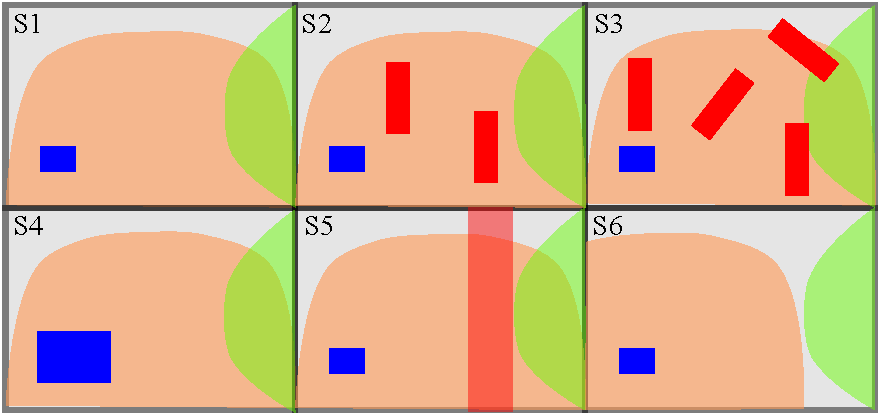
\includegraphics[width=\linewidth]{figures/sces_small.pdf}
\caption{The robot successfully pokes the object (blue) from its reachable workspace (orange) to the goal region (green) in all scenarios while avoiding obstacles (red). \textsl{PokeRRT}, \textsl{PokeRRT*}, and baseline algorithms are evaluated in 6 scenarios---no obstacles (S1), $2$ obstacles (S2), $4$ obstacles (S3), wide object (S4), tunnel (S5), and non-overlapping shared workspace (S6). The robot is unable to i) push or pick-and-place in S6 due to limited robot reach, ii) push in S5 due to workspace obstruction in the action path, and iii) pick-and-place in S4 due to object being wider than gripper width.\vspace{-12pt}}\label{fig:scenarios}
\end{figure}

\subsubsection{Online Path Smoothing}

To minimize the number of pokes and enable poke planning to cover large distances, we combine empirically-derived heuristics with insights from RRT* \cite{karaman2011sampling} to develop \textsl{PokeRRT*} (\cref{algo:pokerrt*}).
RRT* allows for the discovery of new lower-cost paths until the goal region is reached by introducing two additional steps to RRT---choose-parent and rewiring.
In the context of \textsl{PokeRRT*}, choosing the best parent node $q_{min}$ replaces the edge from $q_{near}$ to $q_{new}$ with the edge from $q_{min}$ to $q_{new}$. Planning time for \textsl{PokeRRT*} can be reduced by using a data-driven heuristic to generate $q_{new}'$---instead of applying actions from $\boldsymbol{a_{valid}}$ to get $q_{new}'$, we sample $\Delta q$ from a range of displacements from a dataset of random pokes $\mathcal{D}$.
$q_{new}'$ is then computed as $q_{near} + \Delta q$ in the direction of $q_{rand}$ (\cref{algo:pokerrt*}, Line 4).

Then $q_{min}$ is chosen as the neighbor within radius $r$ of $q_{new}'$ that minimizes the number of pokes from $q_{start}$ to $q_{new}'$ (\cref{algo:pokerrt*}, Line 5). Radius $r$ is selected empirically as the average displacement of the object in the dataset $\mathcal{P}$.
The best action from $q_{min}$ to $q_{new}'$ is recomputed by sampling actions from $\boldsymbol{a_{valid}}$ to make sure each edge in the graph is a valid action. Resultant pose $q_{new}$ is chosen as one that minimizes the distance to $q_{new}'$. $q_{new}$ and the edge from $q_{min}$ to $q_{new}$ are added to the graph.
In the rewiring step, the neighborhood of $q_{new}$ is rewired to minimize the number of pokes along the path from $q_{start}$ through $q_{new}$ to a neighboring leaf node (\cref{algo:pokerrt*}, Lines 8-12). Note that \textsl{PokeRRT*} does not use the extension to RRT* that exploits the anytime nature of RRT* to continuously improve path quality by allocating planning time \cite{karaman2011anytime}---choose-parent and rewiring are the primary modes for online path sparsification.
As a result, \textsl{PokeRRT*} leads to fewer pokes in the planned path than \textsl{PokeRRT}, thereby taking advantage of poking's core competency of allowing larger displacements.

% \begin{algorithm}\small
% \caption{PokeRRT*} \label{alg: pokerrt*}
% \Comment{Choose the best parent node}
% $q_{new} \gets closest(q_{rand}, q_{near} + \Delta q_i) \; \forall \; \Delta q_i$\;
% $q_{best} \gets None$\;
% $num\_pokes \gets$ number of pokes from $q_{start}$ to $q_{new}$\;
% \SmallComment{Find $q_{best}$ (neighbor node of $q_{new}$) with the fewest number of pokes}
% \For{$q$ within radius $r$ of $q_{new}$}{
%     \If{number of pokes from $q_{start}$ to $q + 1 < num\_pokes$}{
%         $q_{best} \gets q$\;
%         $num\_pokes \gets$ number of pokes from $q_{start}$ to $q + 1$\;
%     }
% }
% \SmallComment{Recompute $q_{new}'$ by poking from $q_{best}$}
% $possible\_q_{new}' \gets q_{best} + \boldsymbol{a_{valid}}$\;
% $q_{new}' \gets closest(q_{new}, possible\_q_{best})$\;
% \Comment{Rewiring Step}
% \For{$q$ within radius $r$ of $q_{new}'$}{
%     \If{number of pokes from $q_{start}$ to $q_{new}' + 1 <$ number of pokes from $q_{start}$ to $q$}{
%         set parent of $q$ as $q_{new}'$\;
%     }
% }
% \end{algorithm}


% \begin{figure*}
% \centering
% \includegraphics[width=\linewidth]{figures/sim_table_new.pdf}
% \caption{The robot successfully pokes the object (blue) from its reachable workspace (orange) to the goal region (green) in all scenarios while avoiding obstacles (red). \textsl{PokeRRT}, \textsl{PokeRRT*}, and baseline algorithms are evaluated in 6 scenarios---no obstacles (S1), $2$ obstacles (S2), $4$ obstacles (S3), wide object (S4), tunnel (S5), and non-overlapping shared workspace (S6). The robot is unable to i) push or pick-and-place in S6 due to limited robot reach, ii) push in S5 due to workspace obstruction in the action path, and iii) pick-and-place in S4 due to object being wider than gripper width. See \cref{tab:scenarios} for more detail.\vspace{-10pt}}\label{fig:scenarios}
% \end{figure*}

% \apsout{Then $q_{min}$ is chosen as the neighbor within radius $r$ of $q_{new}$ that minimizes the number of pokes from $q_{start}$ to $q_{new}$.}
% Radius $r$ is selected empirically as the average displacement of the object in a pre-collected dataset of random pokes. The best action from $q_{min}$ to $q_{new}$ is recomputed by sampling actions from $\boldsymbol{a_{valid}}$ to make sure each edge in the graph is a valid action. Resultant pose $q_{new}'$ is chosen as one that minimizes the distance to $q_{new}$. $q_{new}'$ and the edge from $q_{min}$ to $q_{new}'$ are added to the graph.
% In the rewiring step, the neighborhood of $q_{new}'$ is rewired to minimize the number of pokes along the path from $q_{start}$ through $q_{new}'$ to a neighboring node. \ap{Note that \textsl{PokeRRT*} does not use the extension to RRT* that exploits the anytime nature of RRT* to continuously improve path quality by allocating planning time \cite{karaman2011anytime}---choose-parent and rewiring are the primary modes for online path sparsification.}
%As depicted in \cref{fig:plans},
